%&pdflatex
\section{Partizionamento del disco}
Questa è la parte più difficile (e pericolosa). Dobbiamo partizionare il disco per far spazio a Debian. Prima di tutto, bisogna scegliere che partizioni creare per Debian: possiamo farne una sola, che conterrà tutto il sistema operativo, i programmi, e i nostri dati; oppure più partizioni dove, ad esempio, una partizione contiene il sistema operativo e i programmi (partizione \texttt{root}, simbolo \texttt{/}) e un'altra i nostri dati personali (partizione \texttt{/home}); possiamo anche dividere ulteriormente il sistema in altre partizioni ancora (\texttt{/var}, \texttt{/tmp}, \texttt{/usr}, ecc.), ma non lo consigliamo. Nell'esempio di questo testo, divideremo Debian su due partizioni: la \texttt{root} (\texttt{/}) e la \texttt{/home}. Se però si preferisce, è possibile inserire anche tutto in un'unica partizione.

Dobbiamo anche decidere se utilizzare \texttt{LVM}, che permette in qualsiasi momento di ridimensionare le partizioni facilmente (si cerchi sul web per maggiori informazioni); e se cifrare il disco per evitare che qualcuno possa vedere i nostri dati semplicemente avviando una live sul sistema (si cerchi sul web per \textit{"LUKS"} per maggiori informazioni). Anche se è fortemente consigliato cifrare il disco per la sicurezza, la procedura (comunque semplice) non sarà vista in questo testo. Di seguito, ci limiteremo a partizionare il disco senza usare \texttt{LVM} e senza cifrare il disco.

\begin{figure}[ht]
	\centering
	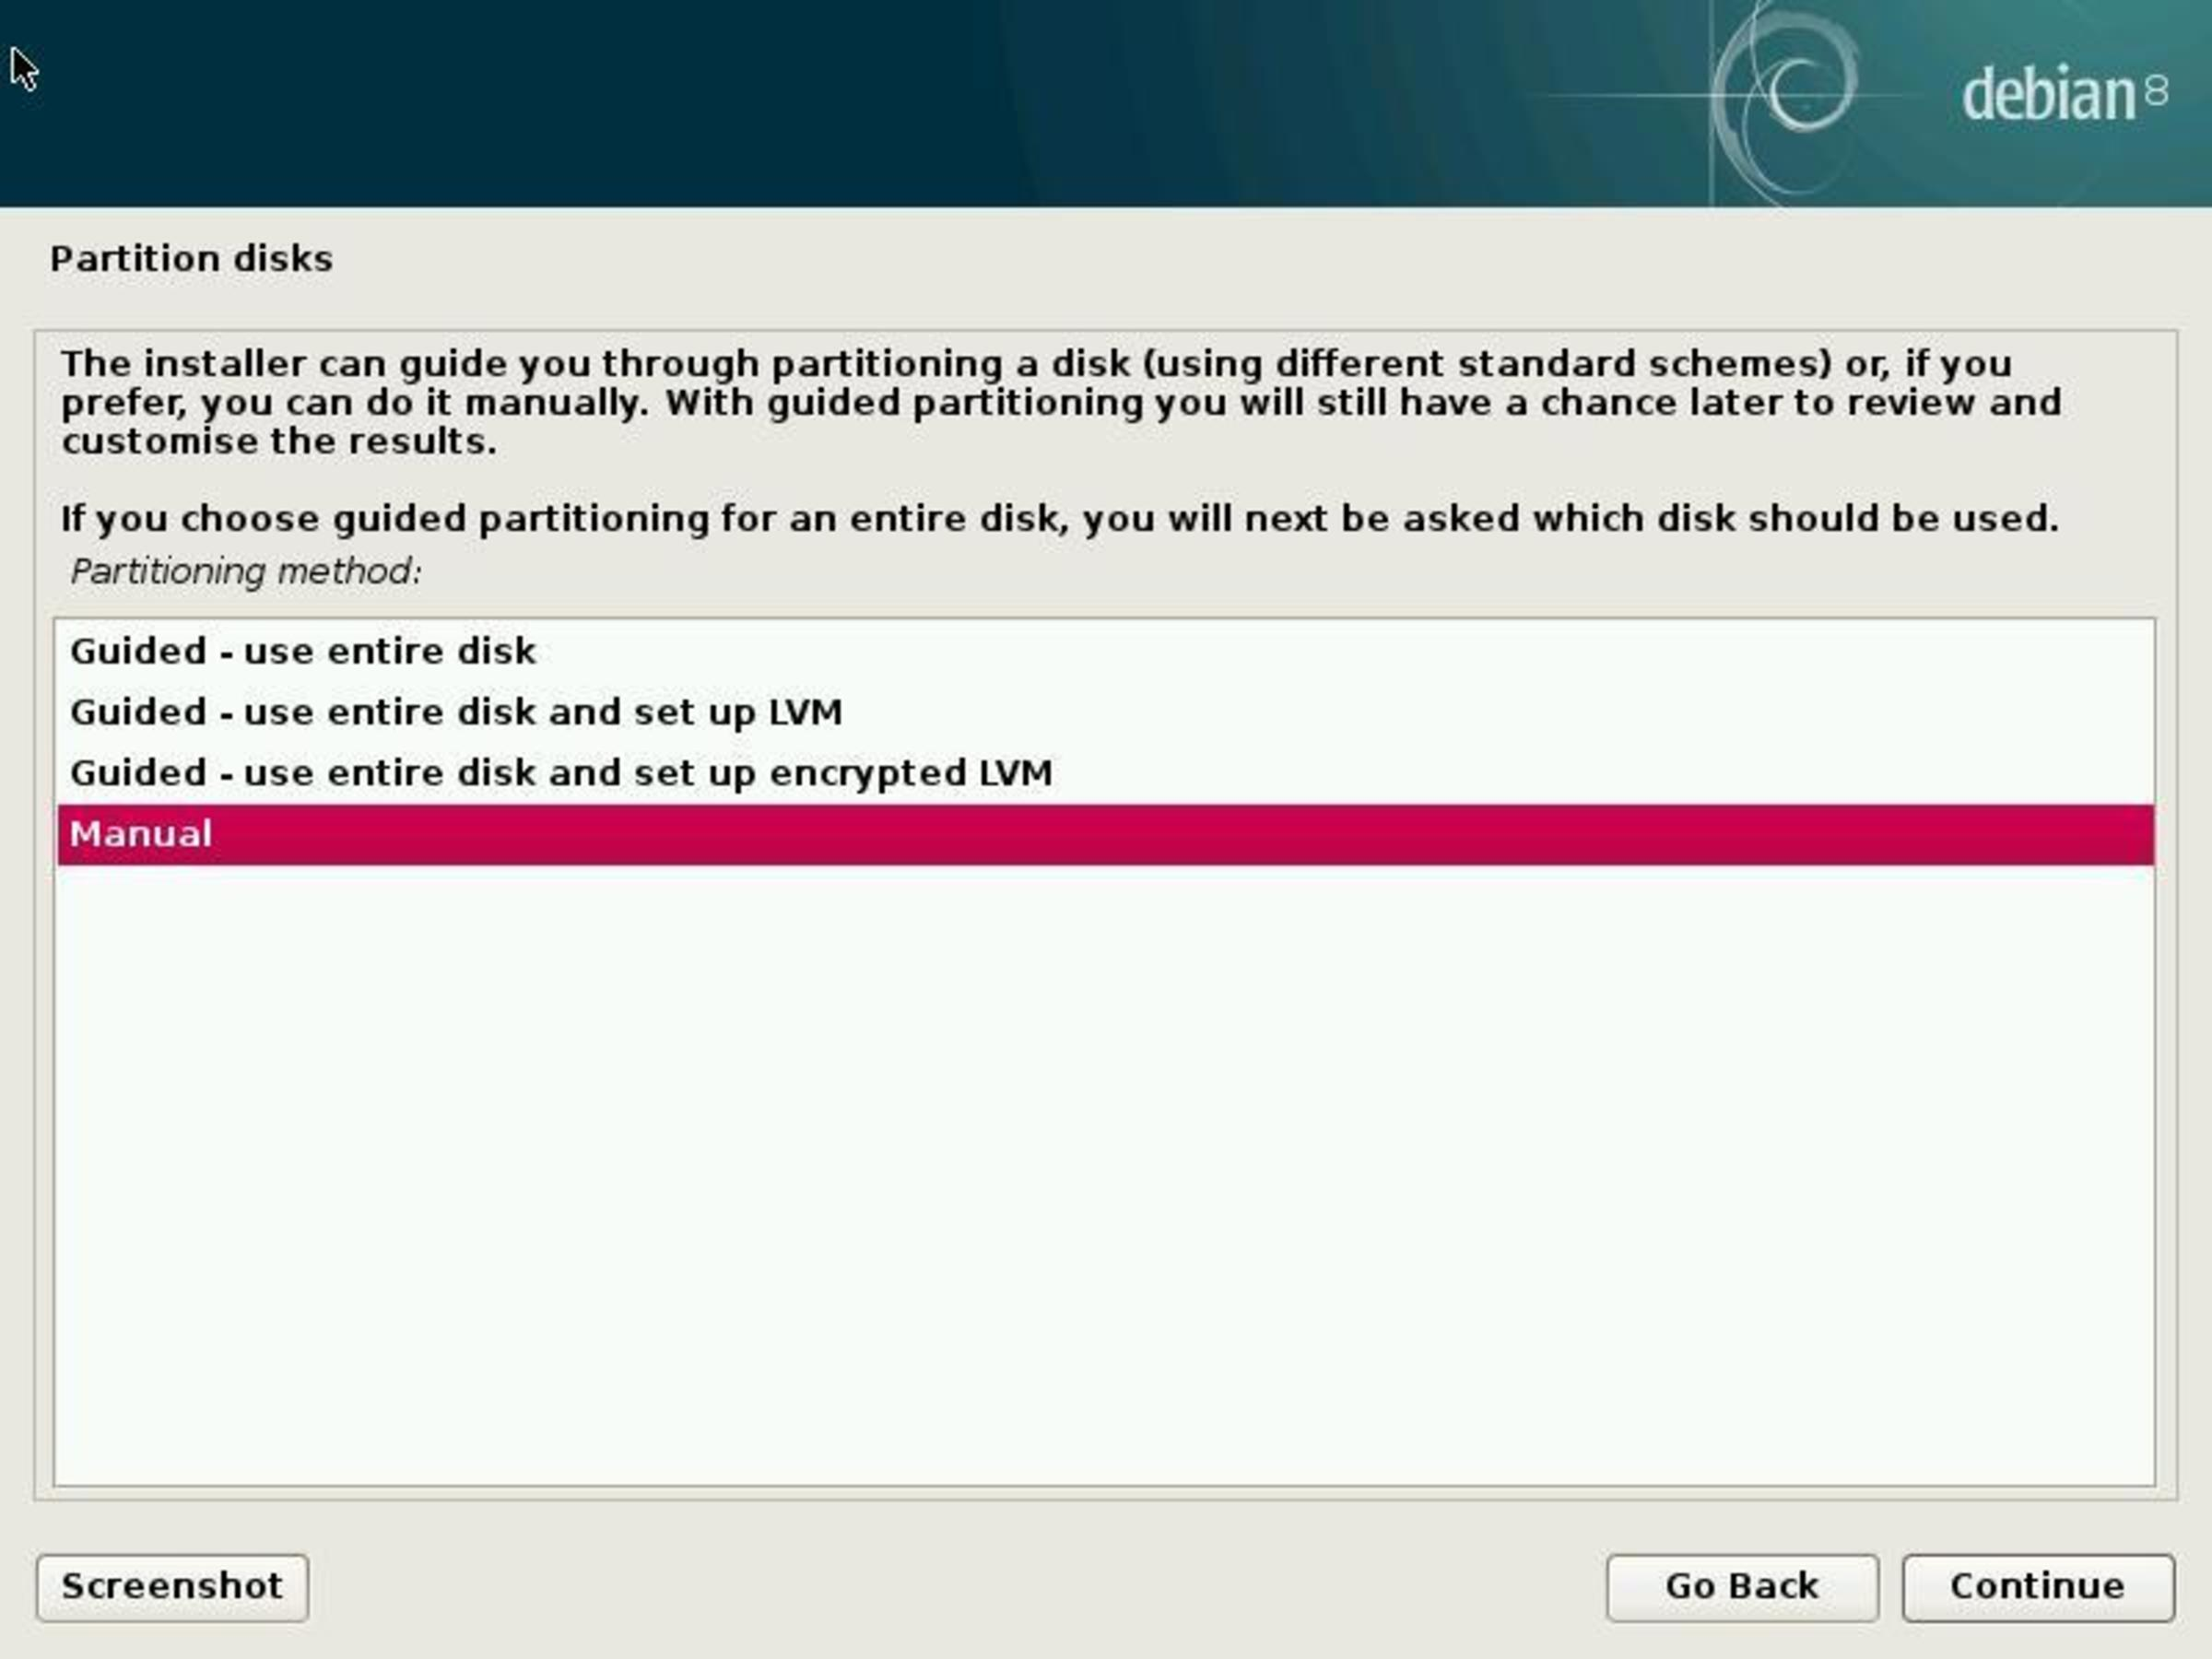
\includegraphics{manual-partitioning}
	\caption{Scelta del metodo di partizionamento: guidato o manuale}
	\label{fig:manual-partitioning}
\end{figure}

Inoltre, a questo punto, dobbiamo decidere se impostare un dual-boot con il sistema operativo già presente sul sistema (nell'esempio, Windows 10), oppure se sostituire il vecchio sistema operativo. Se vogliamo sostituire il vecchio sistema operativo, nella schermata di Figura \vref{fig:manual-partitioning} sceglieremo uno dei tre metodi guidati (\texttt{Guided}), in base al fatto se vogliamo anche impostare \texttt{LVM} e cifrare il disco. Dobbiamo scegliere la procedura guidata anche nel caso di installazione sotto macchina virtuale. Se scegliamo la procedura guidata, successivamente ci ritroveremo direttamente alla schermata di Figura \vref{fig:partitioning}.
Se invece vogliamo mantenere anche il vecchio sistema operativo e configurare un dual-boot, dobbiamo scegliere il metodo di partizionamento \texttt{Manuale} (\texttt{Manual}, in Figura \vref{fig:manual-partitioning}), e ridurre la dimensione della partizione dell'altro sistema operativo per far spazio a Debian.
%&pdflatex
\subsection{Ridimensionare una partizione}
Per ridimensionare una partizione dobbiamo scegliere il partizionamento manuale e, nella schermata successiva, scegliere la partizione da ridimensionare. Nell'esempio, abbiamo selezionato la partizione di Windows 10 (Figura \vref{fig:resize-partition}). Si noti che Windows ha creato 2 partizioni: una da poco più di \texttt{524 MB}, e un'altra da \texttt{53.2 GB} (ovviamente le dimensioni possono essere diverse). La prima partizione (la più piccola) \textbf{non deve essere toccata!}. Se viene modificata, Windows smetterà di funzionare. La seconda partizione (la più grande) è quella che possiamo ridimensionare.

\begin{figure}[ht]
	\centering
	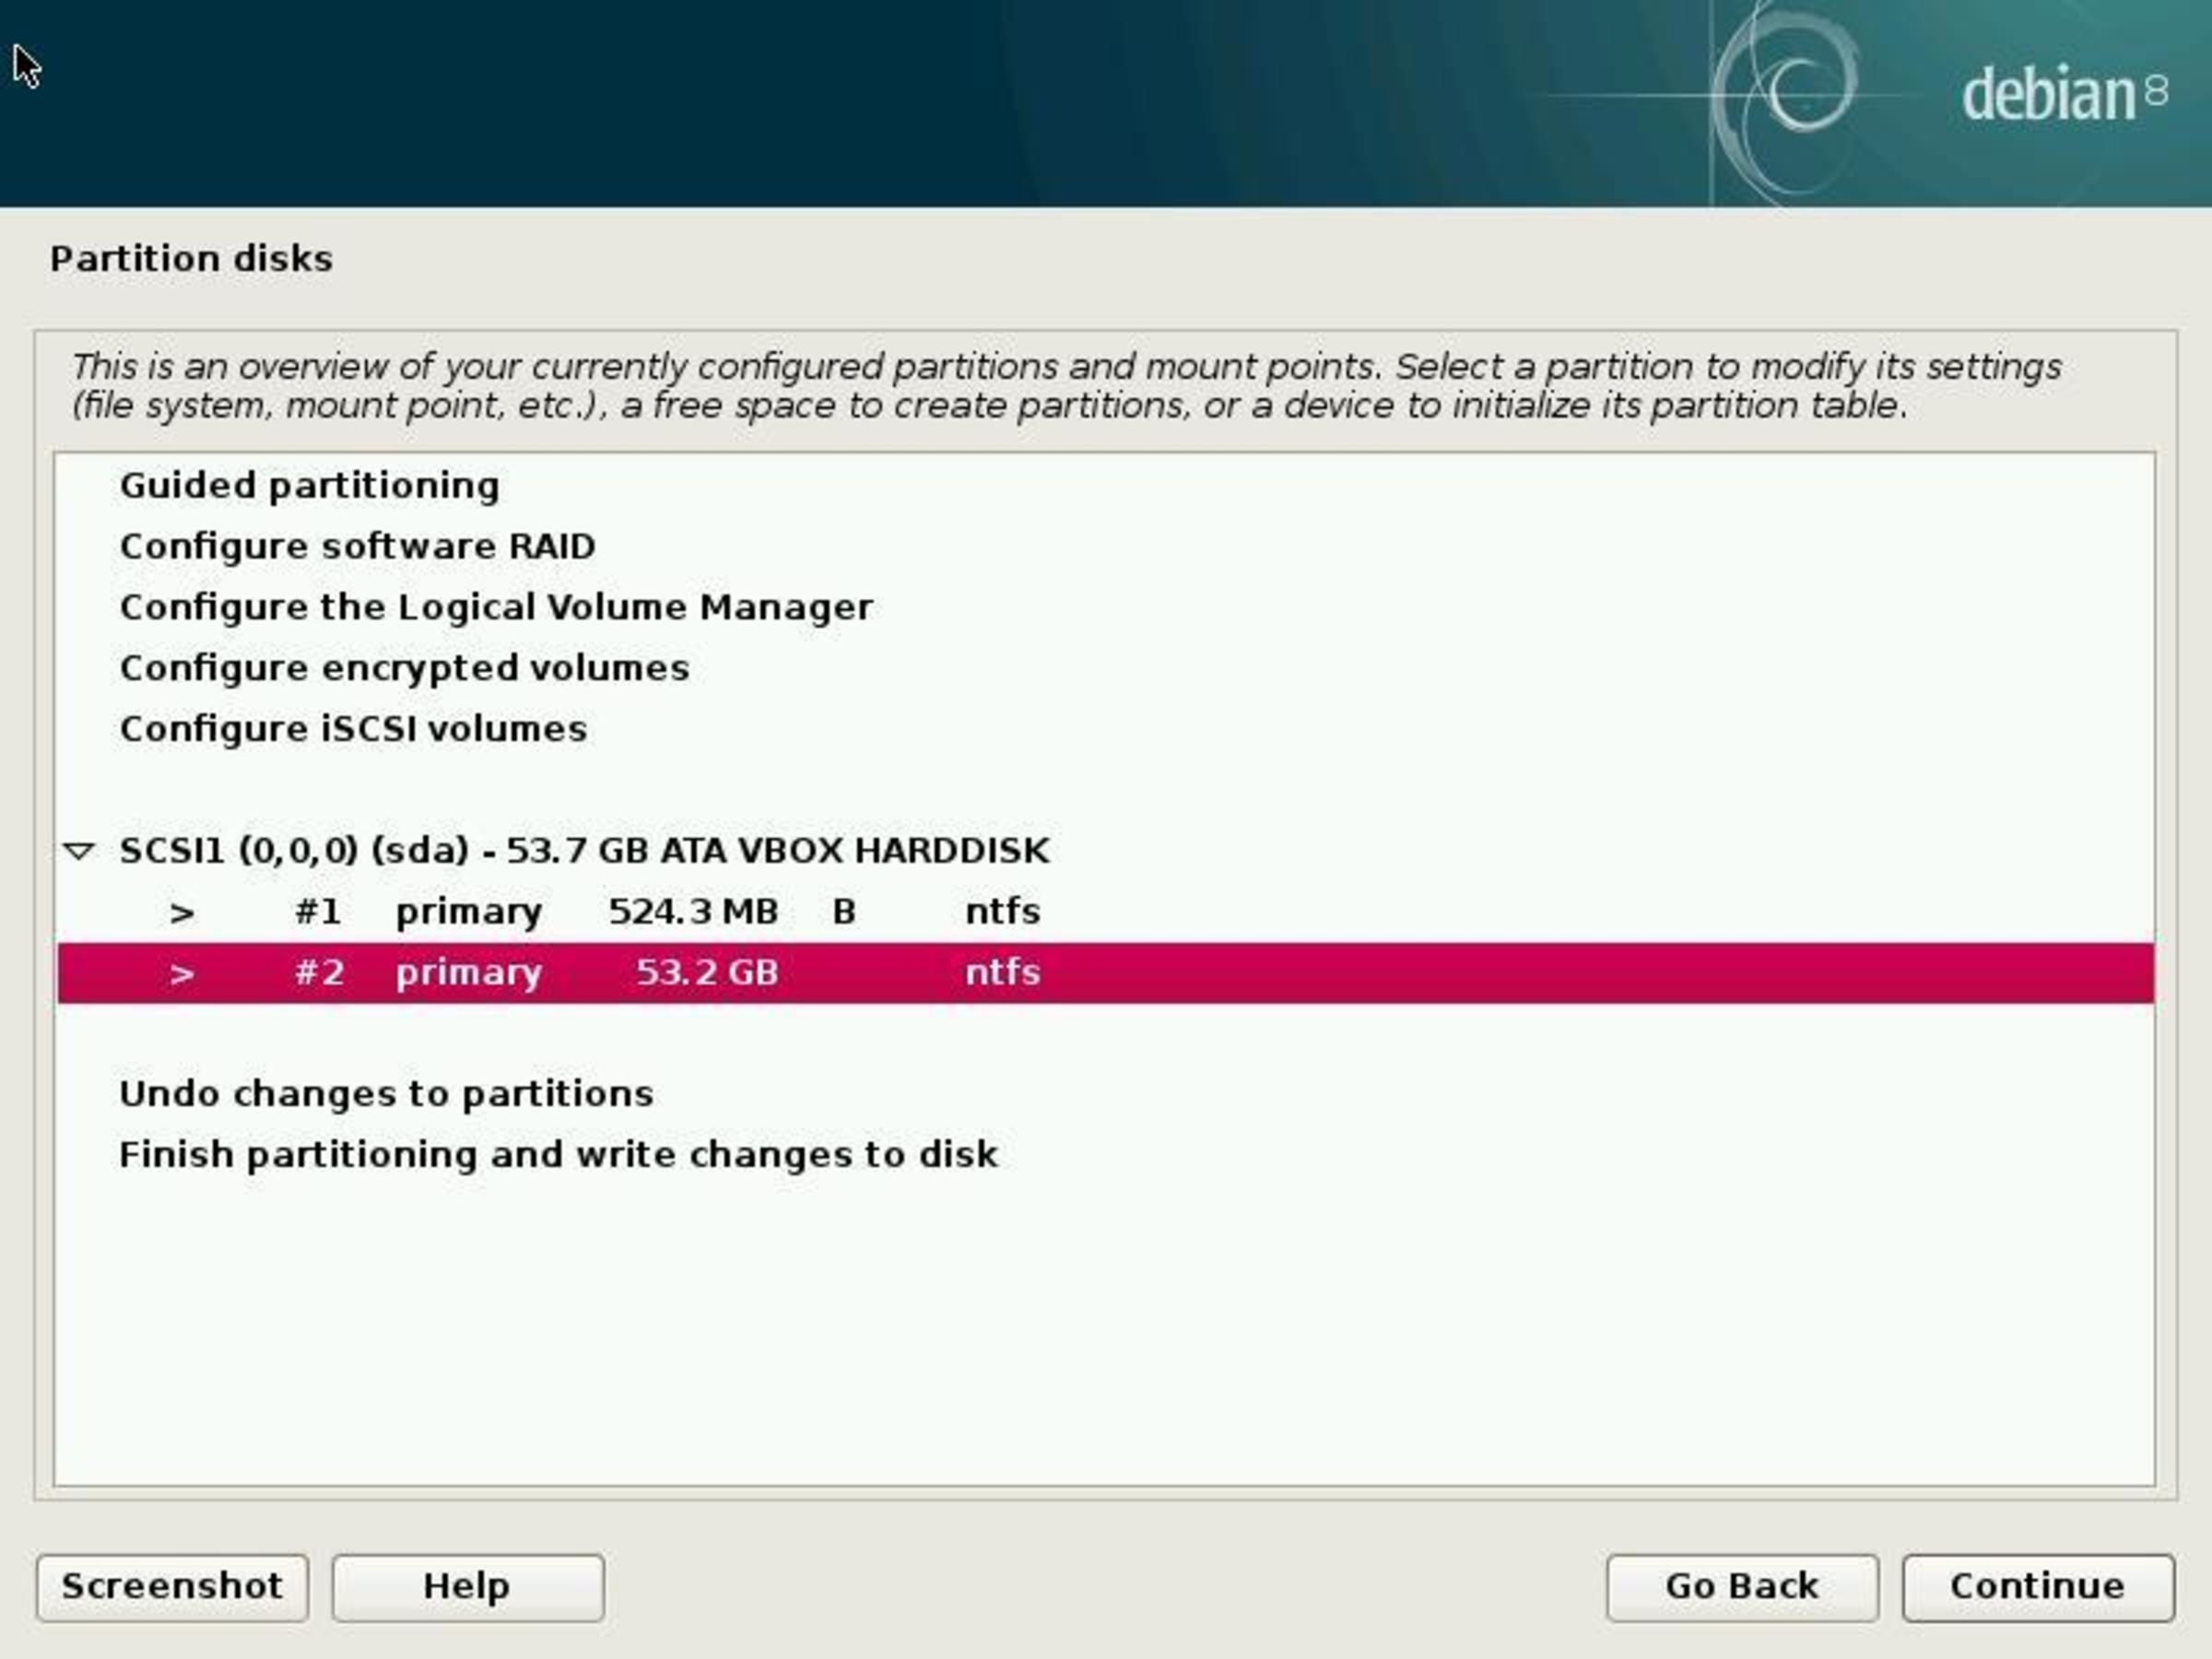
\includegraphics{resize-partition}
	\caption{Selezione della partizione di Windows da ridimensionare}
	\label{fig:resize-partition}
\end{figure}

Dopodiché Debian ci chiederà cosa fare con la partizione selezionata: scegliamo \texttt{Resize the partition} (\texttt{Ridimensionare la partizione}). Quindi ci verrà chiesto di salvare le modifiche fatte finora (anche se non abbiamo ancora fatto nessuna modifica, Debian ce lo chiede comunque): rispondiamo affermativamente con \texttt{Yes} (\texttt{Sì}). Infine, ci verrà chiesta la nuova dimensione per la partizione: consigliamo di riservare almeno \texttt{30 GB} per Debian, e quindi di ridurre la partizione di almeno \texttt{30 GB} rispetto alla dimensione originale.

Al termine ci ritroveremo nella lista delle partizioni: a questo punto dovrebbe essersi generata una quantità di spazio libero sufficiente a contenere Debian (Figura \vref{fig:select-free-space}).

%&pdflatex
\subsection{Partizioni per Debian}
Dobbiamo a questo punto selezionare lo spazio libero sul disco, come in Figura \vref{fig:select-free-space}.

\begin{figure}[ht]
	\centering
	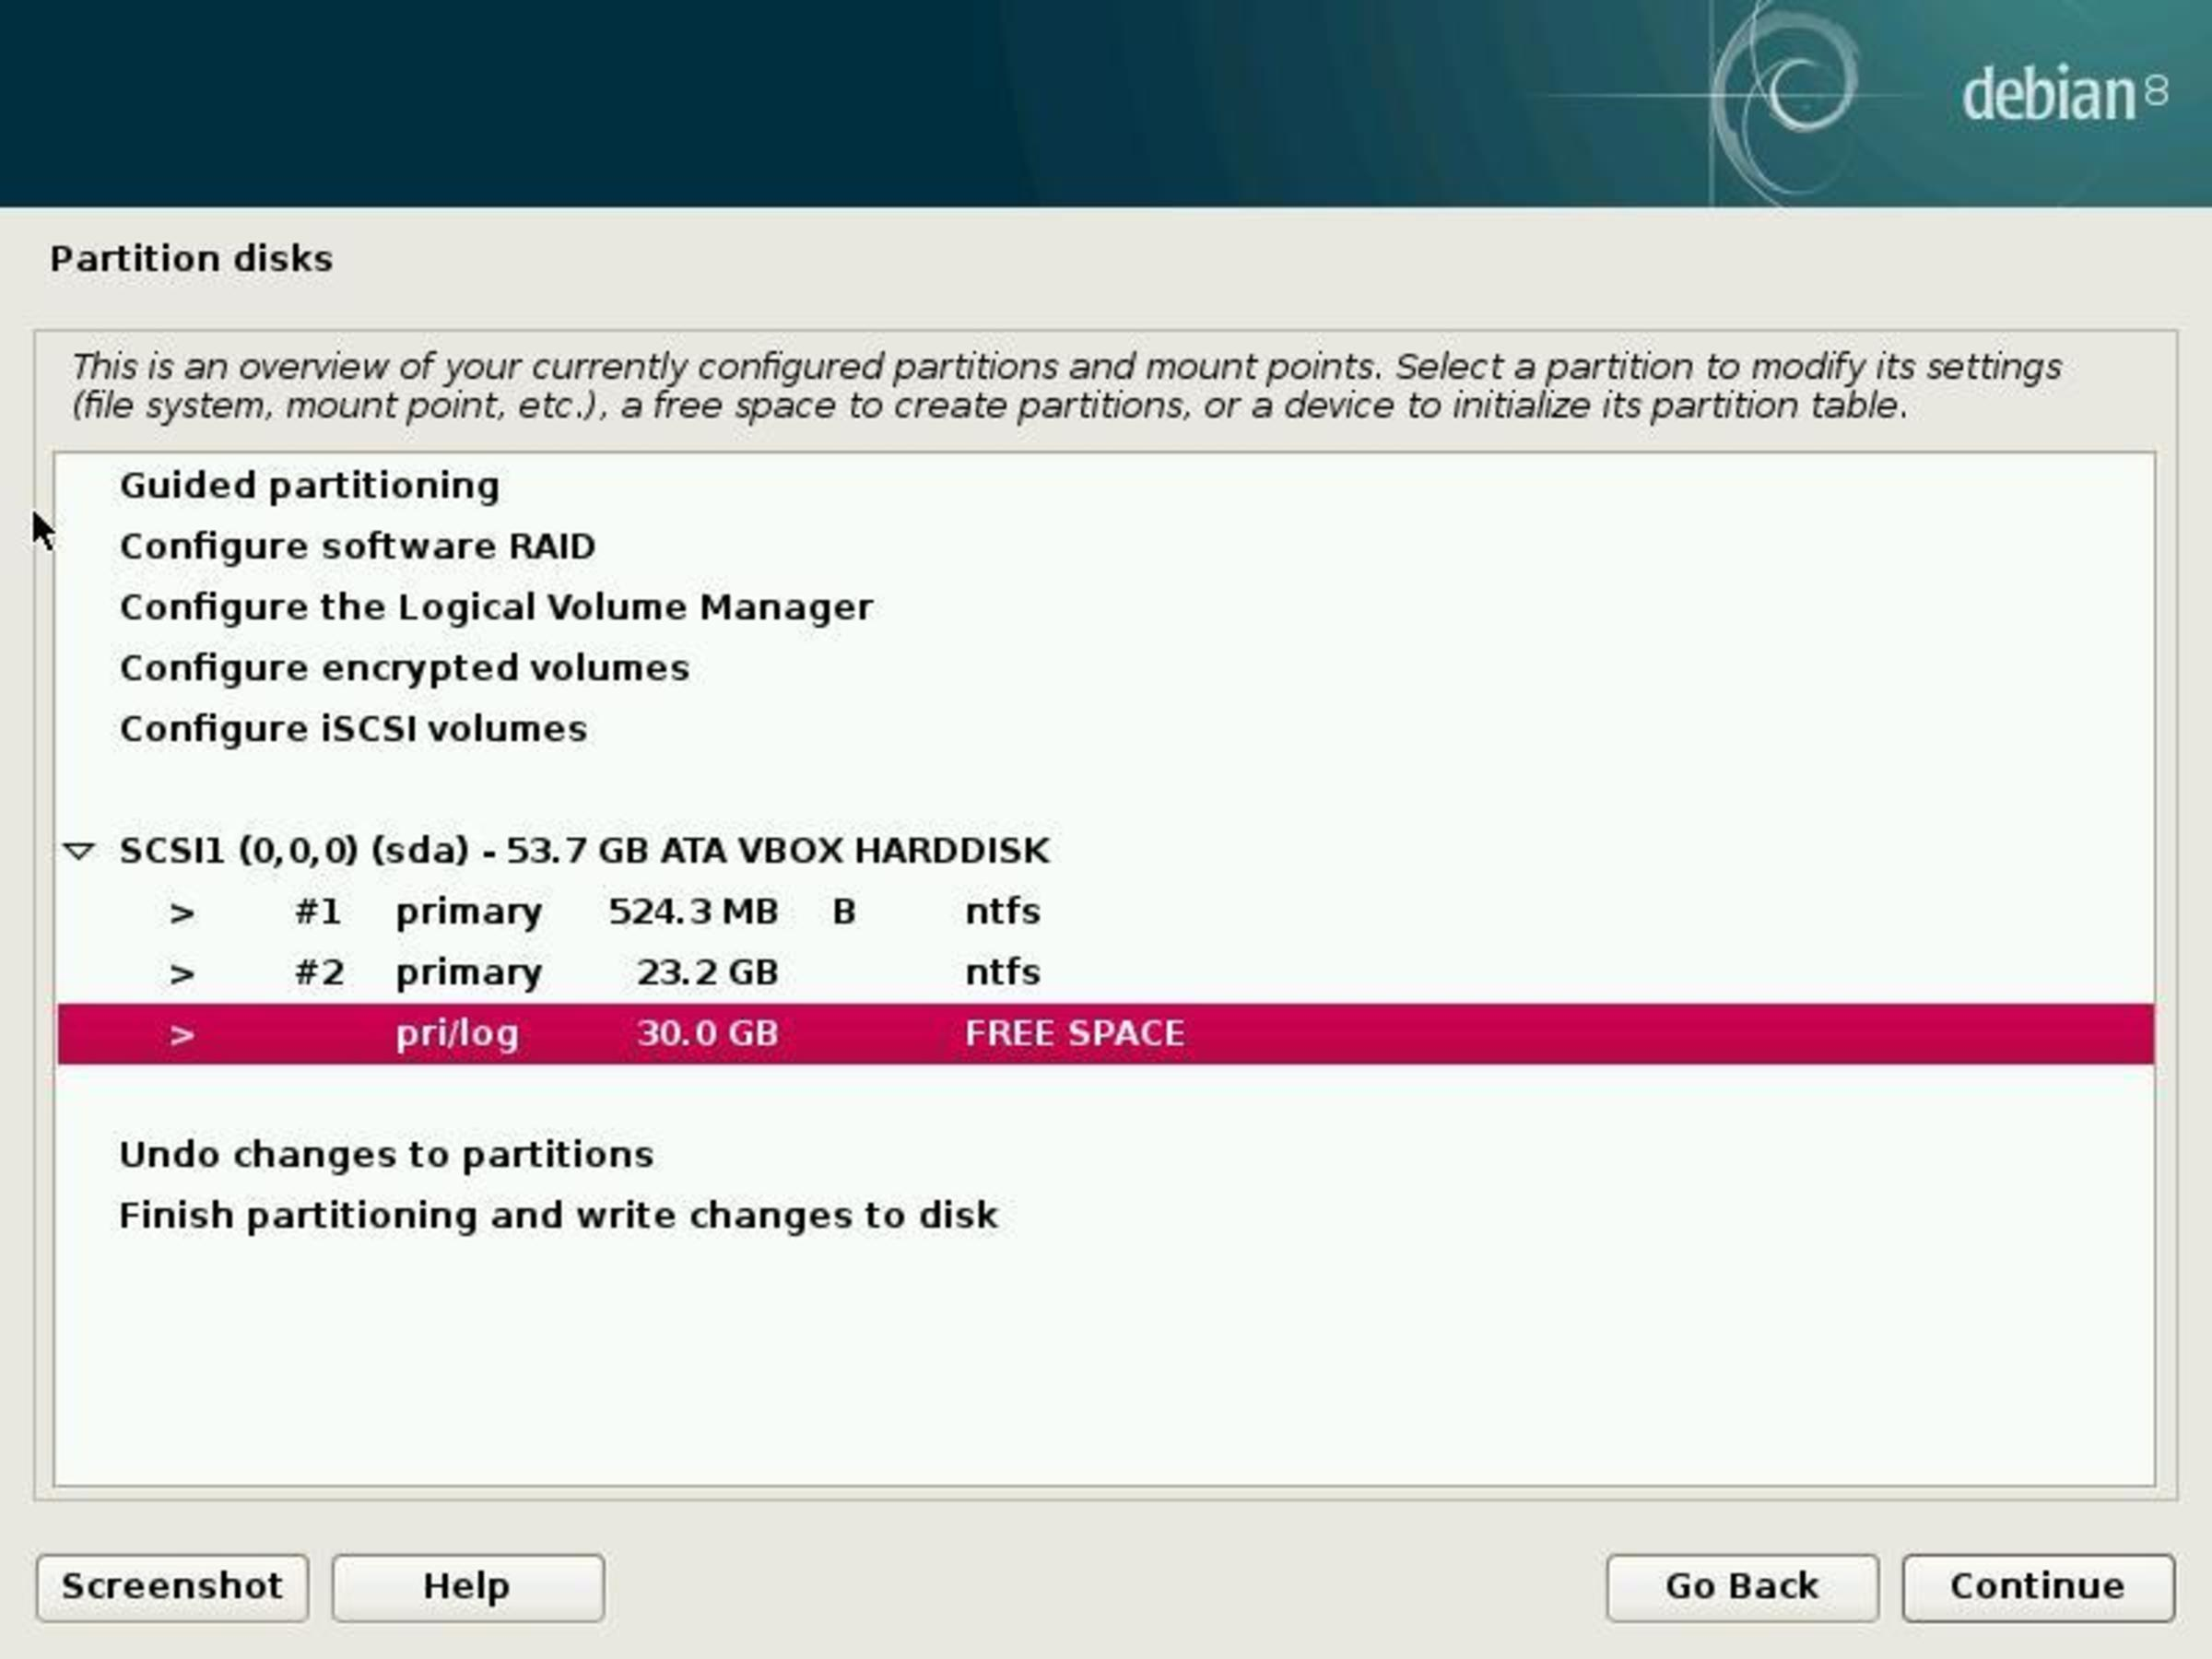
\includegraphics{select-free-space}
	\caption{Selezione dello spazio libero da utilizzare per le partizioni di Debian}
	\label{fig:select-free-space}
\end{figure}

Nella schermata successiva, selezioniamo \texttt{Automatically parti\-tion the free space} (\texttt{Partizionare automaticamente lo spa\-zio libero}). A questo punto saremo ricondotti al partizionamento guidato di Figura \vref{fig:partitioning}. Si scelga il partizionamento preferito (consigliamo di evitare di separare \texttt{/var} e \texttt{/tmp}).

\begin{figure}[ht]
	\centering
	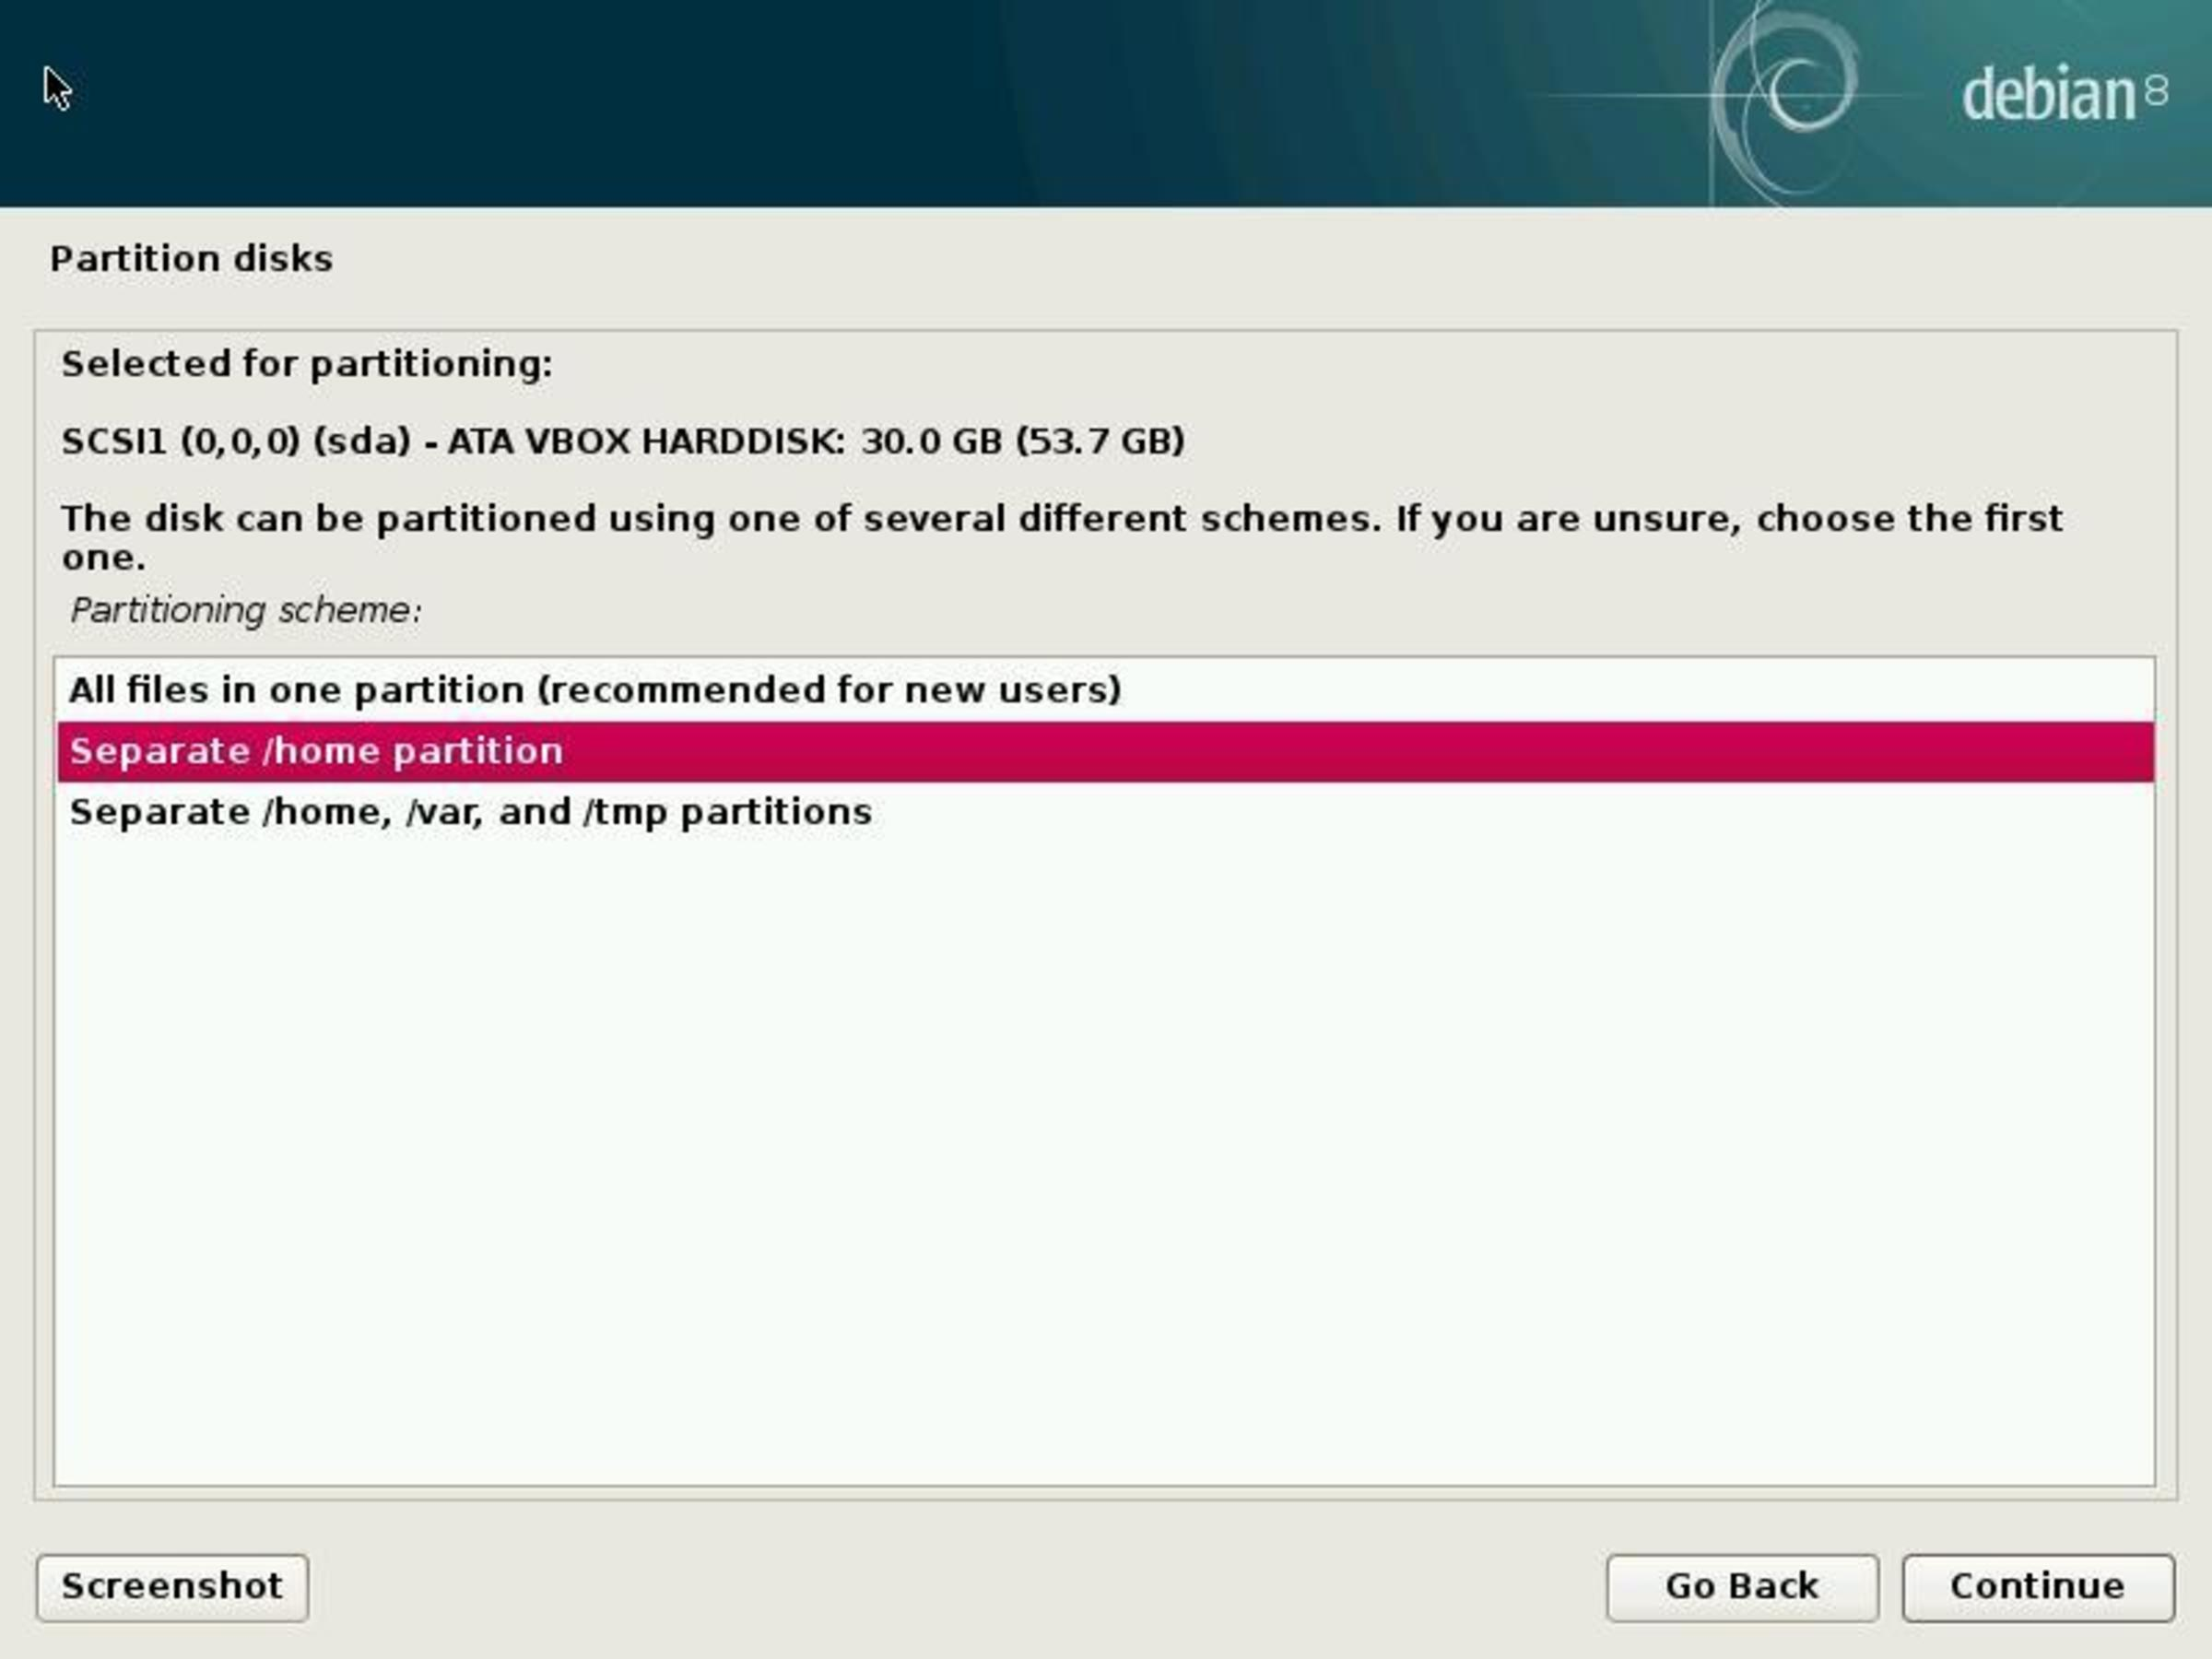
\includegraphics{partitioning}
	\caption{Selezione dello schema delle partizioni con partizionamento guidato}
	\label{fig:partitioning}
\end{figure}

A questo punto Debian ci farà vedere lo schema finale. Selezioniamo quindi \texttt{Finish partitioning and write changes to disk} (\texttt{Terminare il partizionamento e scrivere le modifiche sul disco}). Rispondiamo affermativamente alla domanda di conferma di scrittura delle modifiche su disco. Debian a questo punto salverà le nuove partizioni e inizierà ad installare il sistema di base.

